%%%%%%%%%%%%%%%%%%%%%%%%%%%%%%%%%%%%%%%%%%%%%%%%%%%%%%
\section{A neural-network parametrisation of the zero-loss peak}
%%%%%%%%%%%%%%%%%%%%%%%%%%%%%%%%%%%%%%%%%%%%%%%%%%%%%
\label{sec:methodology}

In this section we present the methodology that will be
used in this work to parametrise and subtract in a model-independent manner
the zero-loss peak present in the low-loss region of EEL spectra.
%
As mentioned in the introduction, our strategy will be inspired in the successful
NNPDF approach used in high-energy physics for the determination of
unpolarised~\cite{Ball:2008by,Ball:2012cx,Ball:2014uwa,Ball:2017nwa}
and polarised parton distributions functions (PDFs) of protons, the nuclear
parton distributions~\cite{AbdulKhalek:2020yuc}, and the fragmentation functions of partons into hadrons.
%
First of add we discuss the parametrisation of the ZLP in terms of neural networks.
%
We then review the estimate and propagation of uncertainties using the MC replica method.
%
Afterwards we present our training strategy both in case of vacuum and of sample spectra,
and discuss how to select the hyper-parameters that appear in the model.


In recent years
machine learning techniques have been deployed in several studies
related to transmission electron microscopy methods
in the context of material science~\cite{Gordon:2020, Zhang:2019, Jany:2017, Ziatdinov:2017}.
%
Representative examples
include the automated identification
of atomic-level structural information~\cite{10.1145/2834892.2834896},
the extraction of chemical information
and defect classification~\cite{doi:10.1021/acsnano.7b07504},
and spatial resolution enhancement
using  using a generative adversarial network~\cite{cite-key}.
%
Our work represents to the best of our knowledge
the first time that neural networks are used as 
 unbiased
background removal interpolators, and combined with Monte Carlo sampling to construct a faithful estimate
of the ML model uncertainties.

\subsection{ZLP parametrisation}
\label{sec:parametrisation}

The starting point of our approach is based on noting that, without any loss of generality, the intensity profile
associated to a given EEL spectrum can be decomposed as
\be
\label{eq:IeelTot}
I_{\rm EEL}(\Delta E) =I_{\rm ZLP}(\Delta E) + I_{\rm inel}(\Delta E) \, ,
\ee
where $\Delta E$ is the measured electron energy loss, $I_{\rm ZLP}$ is the zero-loss peak that receives
contributions both instrumental origin  and from elastic scatterings of the fast electrons with the
nuclei of the sample, and  $I_{\rm inel}(\Delta E)$ contains the contribution from
inelastic scatterings off the electrons of the studied sample.
%
In certain limits it is easy to cleanly disentangle the two contributions: for large $\Delta E$
we know that $I_{\rm ZLP}$ vanishes, while for $\Delta E\simeq 0$ then all emission can be associated to
 the ZLP peak.
%
In this work we are interested in the low-loss region, where $I_{\rm ZLP}$ and $I_{\rm inel}$
are of the same order and thus  care is required to separate them.

Our goal is to construct a parametrisation of $I_{\rm ZLP}$ based on artificial
neural networks, whereby we can extract the relevant inelastic contribution by subtracting the
ZLP background to the measured intensity spectra,
\be
\label{eq:ZLPseparation}
I_{\rm inel}(\Delta E) = I_{\rm EEL}(\Delta E) - I_{\rm ZLP}^{\rm mod)}(\Delta E) \, ,
\ee
and thus be able to exploit the physical information contained in $I_{\rm inel}$ for small $\Delta E$.
%
Further, we want to estimate and propagate all the relevant sources of uncertainty associated
both to the input data and to the subtraction procedure.


As discussed in Sect.~\ref{sec:eels}, the ZLP in EELS depends both
on the value of the electron energy loss $\Delta E$ as well as on the operation
parameters of the microscope, such as the electron beam energy $E_b$ and the exposure time
$t_{\rm exp}$.
%
Therefore we want to construct a multidimensional model which takes all relevant
variables as input.
%
This means that in general Eq.~(\ref{eq:ZLPseparation}) must be expressed as
\be
I_{\rm inel}(\Delta E) = I_{\rm EEL}(\Delta E, E_{b},t_{\rm exp}, \ldots) - I_{\rm ZLP}^{\rm mod)}(\Delta E, E_{b},t_{\rm exp}, \ldots) \, ,
\ee
where we note that by construction the subtracted spectra depends only on $\Delta E$ but not on the microscope
operation parameters.
%
Ideally, the ZLP model should be able to accomodate as many input variables as possible.

Following the NNPDF approach, here we parametrise $I_{\rm ZLP}$ by means of
multi-layer feed-forward artificial neural networks, that is, we express our ZLP model as
\be
\label{eq:ZLPmodelNN}
I_{\rm ZLP}^{\rm (mod)}(\Delta E, E_{b},t_{\rm exp}, \ldots)  = \xi^{(n_l)}_1(\Delta E, E_{b},t_{\rm exp}, \ldots) \, ,
\ee
where $\xi^{(n_l)}_1$ denotes the activation state of the single neuron in the last
of the $n_l$ layers of the network when the $n_I$ inputs $\{ \Delta E, E_{b},t_{\rm exp}, \ldots \}$
are used.
%
The weights and thresholds of this neural network model are then determined
by supervised learning regression from a suitable training dataset, as
detailed below.
%
Multi-layer feed forward neural networks benefit from the ability
to parametrise multidimensional input data with arbitrarily
non-linear dependencies: even with a single hidden layer, neural networks
can reproduce general functional dependencies provided one has a large enough
number of neurons.

An schematic representation of our model
is displayed in Fig.~\ref{fig:architecture}.
%
 The input is an $n_I$ array containing $\Delta E$ and the
 operation variables of the microscope, and
 the output is the value of the intensity of the zero-loss peak
 expected for an EEL spectrum for the chosen input variables.
 %
 We adopt an $n_I$-10-15-5-1 architecture with three hidden layers, for a total
 number of 289~(271) free parameters for $n_i=3$~($n_I=1$) to be adjusted by the optimisation procedure.
 %
 We use a sigmoid activation function for the three hidden layers and a ReLU
 for the final one.
 %
 The choice of ReLU for the final layer guarantees that our model for the ZLP
 is positive-definite, as required by general physical considerations.
 %
 We have adopted a redundant architecture  to ensure that the ZLP parametrisation
 is sufficiently flexible, and we avoid over-fitting by means of
 a suitable regularisation strategy, see Sect.~\ref{sec:training}.
  
%%%%%%%%%%%%%%%%%%%%%%%%%%%%%%%%%%%%%%%%%%%%%
\begin{figure}[t]
    \centering
    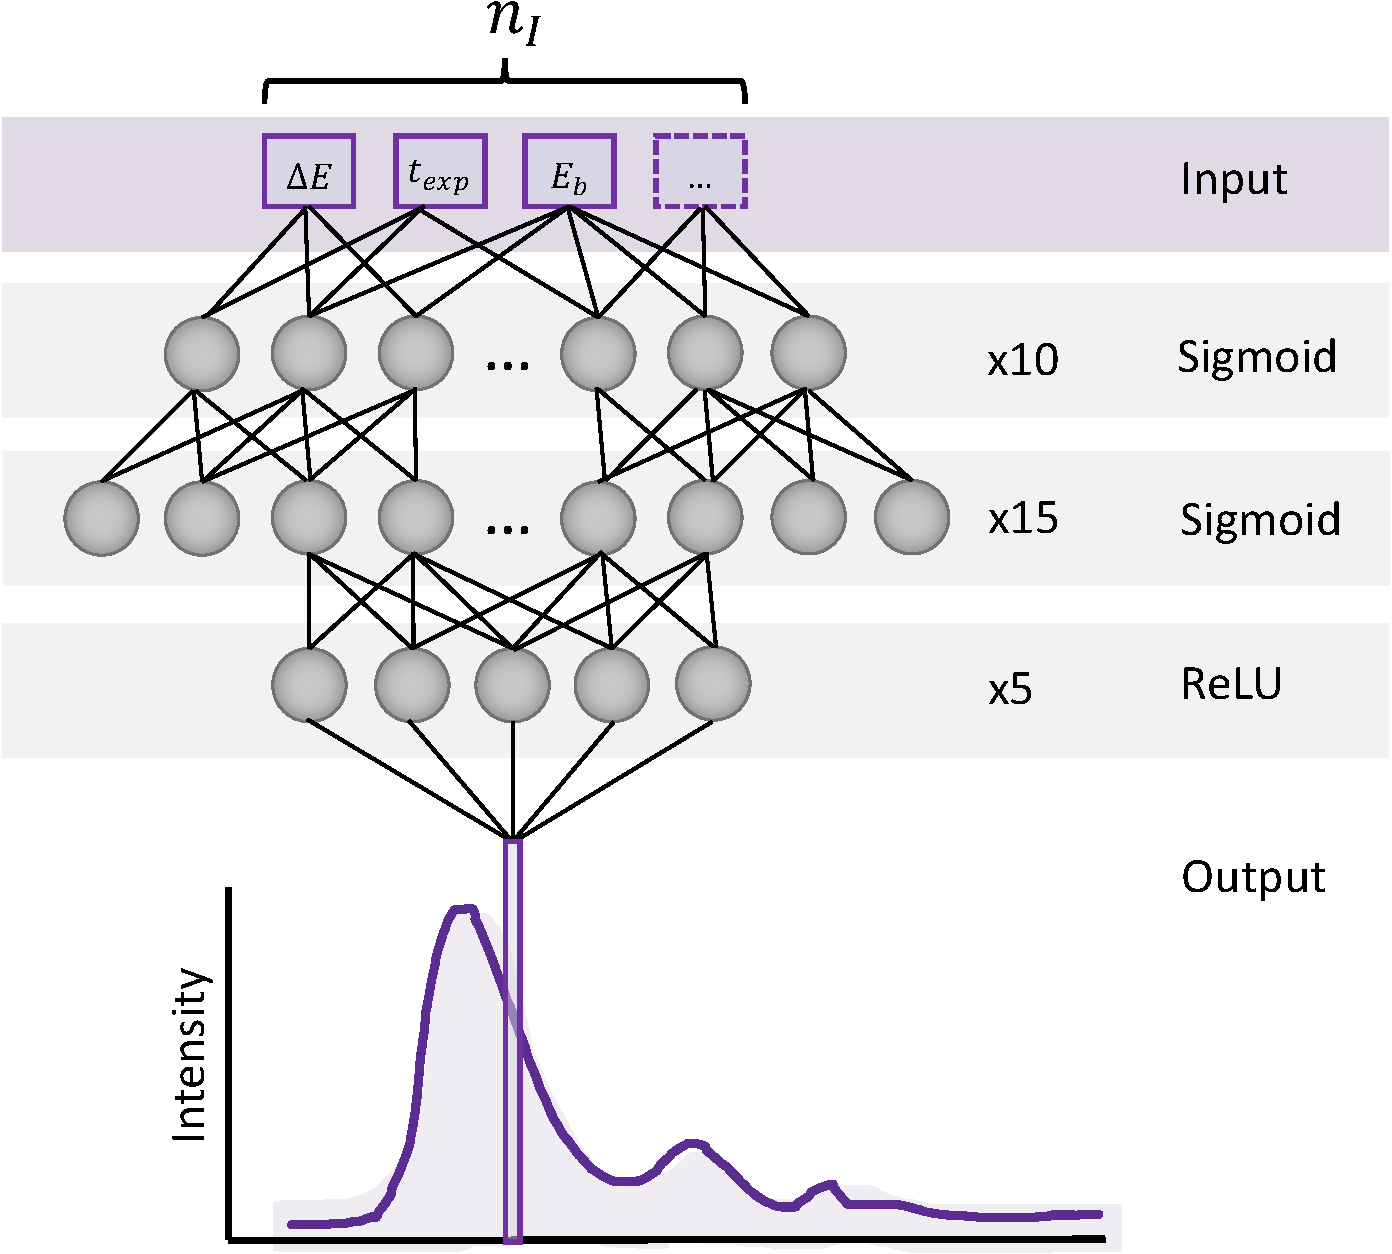
\includegraphics[width=99mm]{plots/architecture.pdf}
    \caption{Schematic representation of the NN-based model of the ZLP used
      in this work, Eq.~(\ref{eq:ZLPmodelNN}).
      %
      The input is an $n_I$-dimensional array containing $\Delta E$ and all other relevant
      operation variables of the microscope such as $E_b$ and $t_{\rm exp}$.
      %
      The output is the predicted value of the intensity of the zero-loss peak
      expected for an EEL spectrum with those specific input variables.
    }
    \label{fig:architecture}
\end{figure}
%%%%%%%%%%%%%%%%%%%%%%%%%%%%%%%%%%%%%%%%%%%%%%%%%

%One of the reasons for the widespread success of machine learning 
%is the growing availability of high processing capabilities 
%and the large amounts of data at disposal~\cite{LeCun:2015}.
%
%Typical machine learning algorithms are divided into three classes:
%supervised learning, unsupervised learning and reinforcement learning~\cite{Kotsiantis:2007}.
%
%A supervised learning regression tool of a feed-forward neural network 
%was chosen for the purpose of this study. This is the simplest type 
%in the group of neural networks and it was selected for its ability
%to it accomodate multidimensional input data and 
%incorporate non-linear interactions, within reasonable computation times. 
%
%For predicting the properties of the ZLP in vacuum, we construct an multidimensional
%input neural network, a schematic of which can be observed in figure~\ref{fig:architecture}.

\subsection{Uncertainty propagation}

Even for EEL spectra taken at identical operation conditions of the microscope,
in general the resulting ZLP intensities will be different as discussed
in Sect.~\ref{sec:eels}.
%
Further, there exist a large number of different NN configurations, each
representing a different functional form for $I_{\rm ZLP}^{(\rm mod)}$ which provide
an equally valid description of the input data.
%
Using the notation of~\cite{Ball:2014uwa} we denote these two types of uncertainties
as the ``experimental'' and ``parametrization'' components.
%
To faithfully estimate these uncertainties and to propagate them to our  predictions
for the ZLP-subtracted spectra without the need of any kind of approximation,
we adopt here the Monte Carlo replica method.
%
The basic idea of this method is to exploit the available information
on experimental measurements (central values, uncertainties, and correlations)
to construct a sampling of the probability density in the space of 
the data, which following the neural network training is propagated
to the probability density in the space of $I_{\rm ZLP}$ models.

%With artificial neural networks as unbiased interpolators to describe the ZLP, 
%it is possible to construct a probability distribution in the space of 
%the experimental data and a faithful estimate of the ML model uncertainties.
%
%This sampled ZLP prediction can be applied to subtract to the EEL spectra while
%keeping full track of all uncertainties associated to the data, model and parametrisation.
%
%Based on the NNPDF approach, 
%error propagation from experimental data to the fit is performed by the Monte Carlo (MC)
%replica method. 
%
%In the MC approach, any statistical property of the ZLP can be derived from a 
%sample of replicas of the function.

Let us assume that we have $n_{\rm dat}$ independent measurements of the ZLP intensity, for
different or the same values of the input parameters collectively denoted as $\{z_i\}$:
\be
I^{\rm (exp)}_{{\rm ZLP},i}\lp \{ z_i  \}\rp = I^{\rm (exp)}_{{\rm ZLP},i}\lp  \Delta E_i, E_{b,i}, t_{\rm exp,i},\ldots \rp
\,, \quad i=1,\ldots,n_{\rm dat} \, .
\ee
The Monte Carlo method is based on the generation
of a large number $N_{\rm rep}$ of Monte Carlo replicas of these original data points
by means of a multi-Gaussian distribution with the central values and covariance matrices
taken from the data,
\be
\label{eq:MCreplicaGen}
  I_{{\rm ZLP},i}^{{\rm (art)}(k)}  =  I^{\rm (exp)}_{{\rm ZLP},i} + r_i^{({\rm stat},k)}\sigma_i^{\rm (stat)}
  + \sum_{j=1}^{n_{\rm sys}} r_{i,j}^{({\rm sys},k)} \sigma_{i,j}^{\rm (\rm sys)} \,, \quad \forall i
  \,, \quad k=1,\ldots,N_{\rm rep} \,.\,\, \,
  \ee
  where $\sigma_i^{\rm (stat)}$ and $\sigma_{i,j}^{\rm (\rm sys)}$ represent the statistical
  and systematic uncertainties (the latter divided into  $n_{\rm sys}$ fully point-to-point correlated
  sources) and $\{r_i^{(k)}\}$ are Gaussianly distributed random numbers.
  %
  The values of $\{r_i^{(k)}\}$ are
  generated with a suitable correlation pattern to ensure
  that averages over the set of Monte Carlo
  replicas reproduce the original experimental covariance matrix,
  \bea
  \la  \lp I_{{\rm ZLP},i}^{{\rm (art)}(k)} - \la I_{{\rm ZLP},i}^{{\rm (art)}(k)}\ra_{\rm rep}\rp
  \lp I_{{\rm ZLP},j}^{{\rm (art)}(k)} - \la I_{{\rm ZLP},j}^{{\rm (art)}(k)}\ra_{\rm rep}\rp\ra_{\rm rep} \nonumber \\ \label{eq:expcovariance} \qquad\qquad = {\rm cov}^{(\rm exp)}\lp I_{{\rm ZLP},i},I_{{\rm ZLP},j}\rp \qquad \, .
  \eea
We thus note that each $k$-th replica contains 
as many data points as the original set.

In the present case, the information on experimental correlations is not accessible and
thus we assume that there is a single source of point-by-point uncorrelated systematic
uncertainty, denoted as $\sigma_i^{\rm (exp)}$, which is estimated as follows.
%
The input measurements will be composed in general on subsets of EEL
spectra taken with identical operation conditions.
%
Assume that for a specific set of operation conditions we have $N_{\rm sp}$ of such spectra.
%
Since the values of $\Delta E$ will be different in each case, first of all
we uniformise a common binning in $\Delta E$ with $n_{\rm dat}$ entries.
%
Then we evaluate the total experimental uncertainty in one of these bins as
\be
\label{eq:sigmaiexp}
\sigma_i^{\rm (exp)} = \lp \frac{1}{N_{\rm sp}-1} \sum_{l=1}^{N_{\rm sp}}
\lp I_{{\rm ZLP},i}^{ ({\rm exp}),l}  - \la I_{{\rm ZLP},i}^{ ({\rm exp})}\ra \rp \rp^{1/2} \, ,
i=1,\ldots, n_{\rm dat} \, ,
\ee
that is, as the standard deviation over the $N_{\rm sp}$ spectra.
%
This uncertainty is separately evaluated for each set of microscope operation conditions
for which spectra are available.
%
In this case, Eqns.~(\ref{eq:MCreplicaGen}) and~(\ref{eq:expcovariance}) reduce to
\be
 I_{{\rm ZLP},i}^{{\rm (art)}(k)}  =  I^{\rm (exp)}_{{\rm ZLP},i} + r_i^{({\rm tot},k)}\sigma_i^{\rm (exp)}
 \,, \quad \forall i
  \,, \quad k=1,\ldots,N_{\rm rep} \,.\,\, \,
\ee
and
  \bea
  \la  \lp I_{{\rm ZLP},i}^{{\rm (art)}(k)} - \la I_{{\rm ZLP},i}^{{\rm (art)}(k)}\ra\rp
  \lp I_{{\rm ZLP},j}^{{\rm (art)}(k)} - \la I_{{\rm ZLP},j}^{{\rm (art)}(k)}\ra\rp\ra_{\rm rep} =
  \sigma_i^{\rm (exp)}\sigma_j^{\rm (exp)}\delta_{ij}
  \eea
given that the experimental covariance matrix is diagonal.  

The value of the number of generated MC replicas, $N_{\rm rep}$, should be chosen such that the set of replicas 
models accurately the probability distribution of original training data.
%
To verify that this is the case,
Fig.~\ref{fig:MC} displays a comparison between the original experimental central values
$I_{{\rm ZLP},i}^{\rm (exp)}$ (left panel) and the corresponding 
uncertainties $\sigma_i^{(\rm exp)}$ with the results of averaging over
a sample of $N_{\rm rep}$ Monte Carlo replicas generated by means of
Eq.~(\ref{eq:MCreplicaGen}) for different number of replicas.
%
We find that $N_{\rm rep}=500$ is a value that ensures that both
the central values and uncertainties are reasonably well reproduced,
and we adopt it in what follows.

%%%%%%%%%%%%%%%%%%%%%%%%%%%%%%%%%%%%%%%%%%%%%%%
\begin{figure}[t]
    \centering
    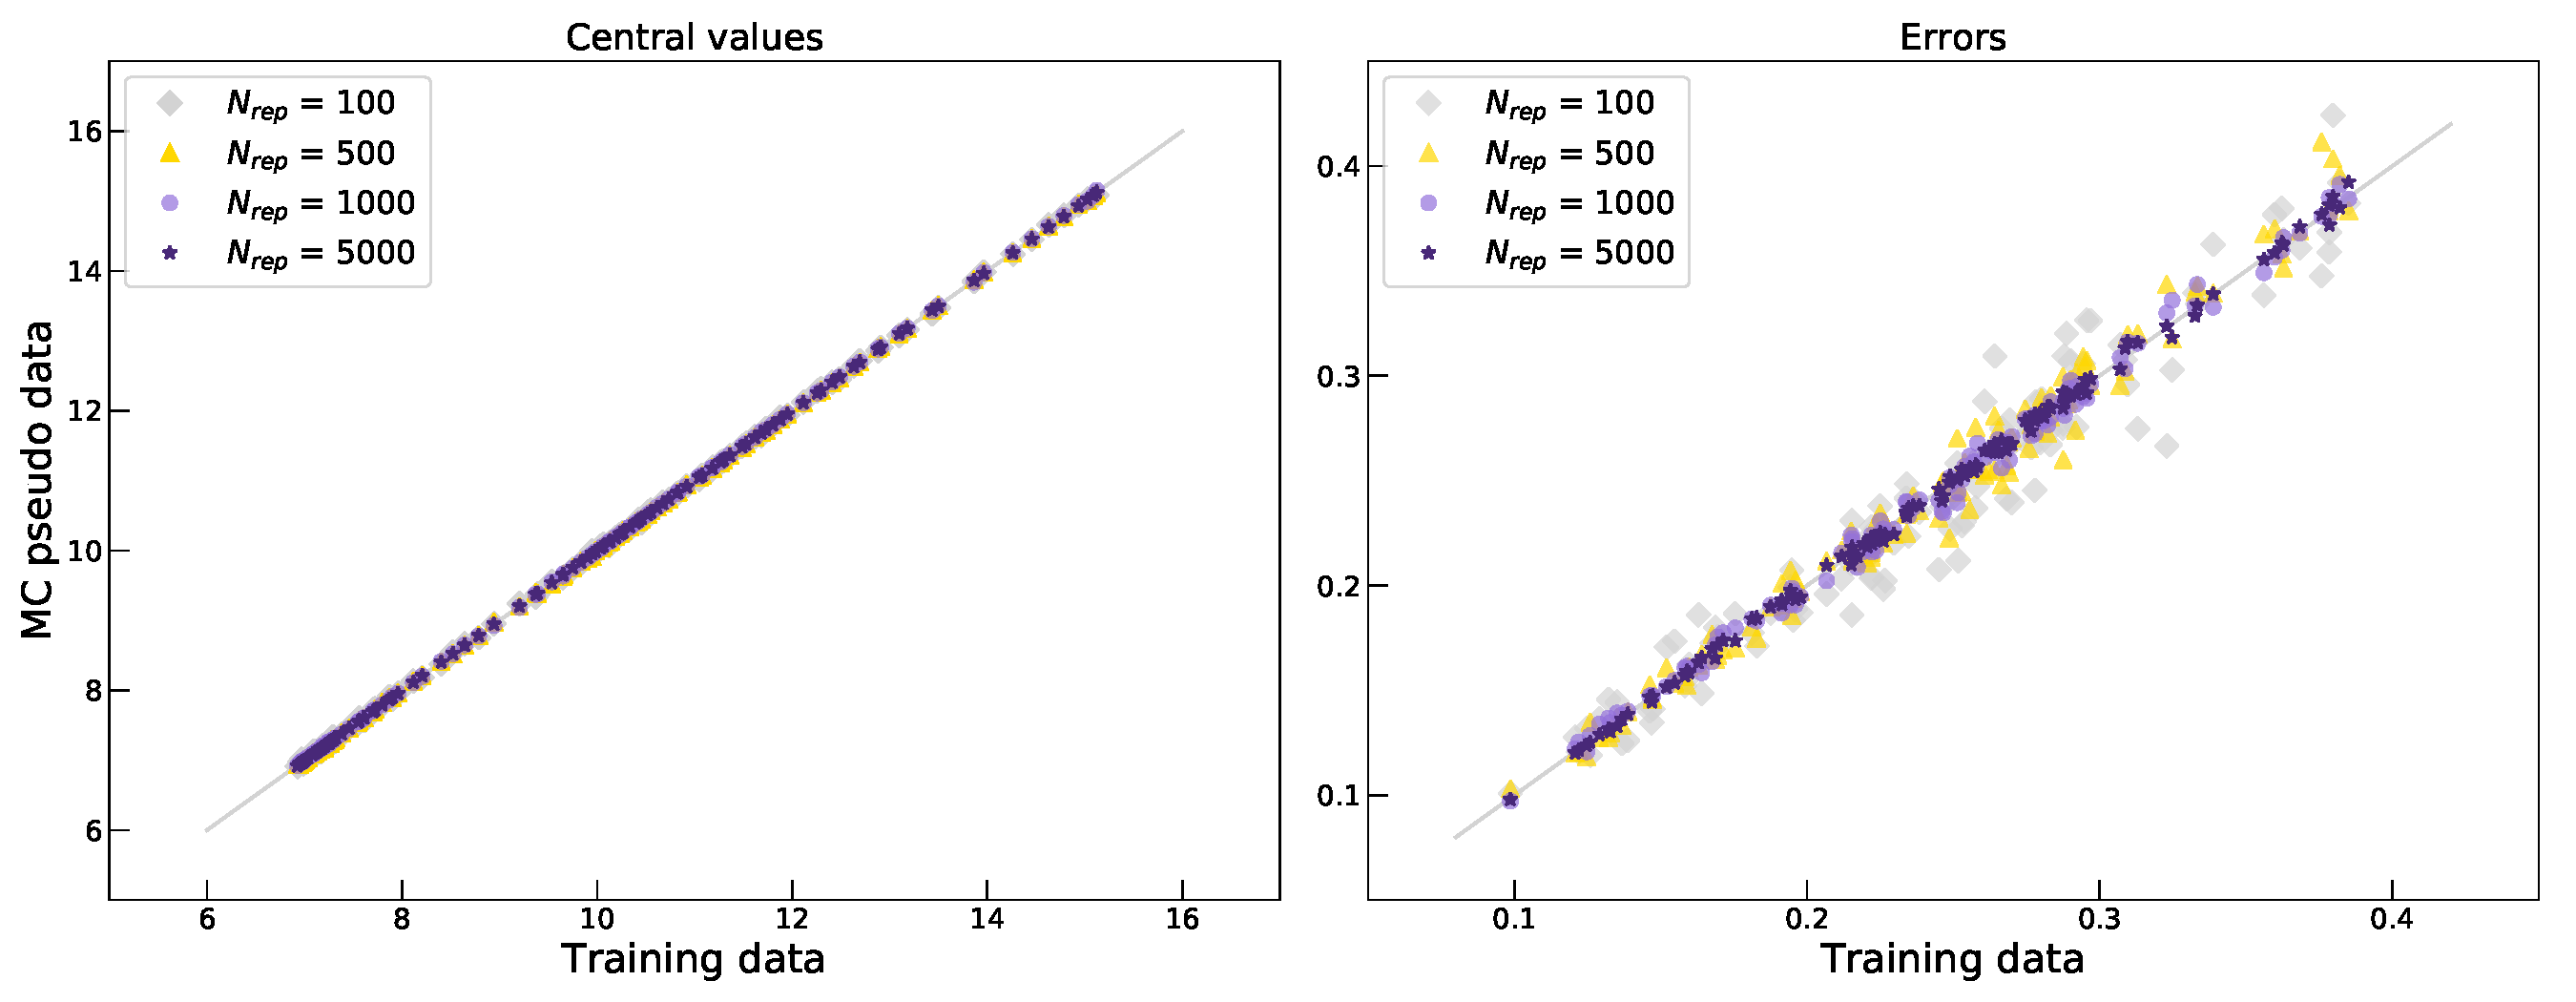
\includegraphics[width=0.99\textwidth]{plots/MC.pdf}
    \caption{Comparison between the original experimental central values
      $I_{\rm ZLP,i}^{\rm exp}$ (left panel) and the corresponding statistical
      uncertainties $\sigma_i^{(\rm stat)}$ with the results of averaging over
      a sample of $N_{\rm rep}$ Monte Carlo replicas generated by means of
      Eq.~(\ref{eq:MCreplicaGen}), for different values of
      $N_{\rm rep}$.
      }
    \label{fig:MC}
\end{figure}
%%%%%%%%%%%%%%%%%%%%%%%%%%%%%%%%%%%%%%%%%%%%%%%%5

\subsection{Training strategy}
\label{sec:training}

The training of the neural-network model for the ZLP peak differs between
the cases of EEL spectra taken on vacuum, where by construction $I_{\rm EEL}(\Delta E) =I_{\rm ZLP}^{\rm (mod)}(\Delta E)$,
and for spectra taken on sample.\footnote{Actually EEL spectra taken in the vacuum but close
  to the sample might still receive inelastic contributions due to processes such as .... Here
  when we use vacuum spectra we consider exclusively those taken reasonably far from the surface
of the analysed nanostructures.}
%
In the latter case, as indicated by Eq.~(\ref{eq:ZLPseparation}), in order to avoid
biasing the results it is
important to ensure that the model is trained only on the region of the spectra
where the ZLP dominates over the inelastic scatterings.
%
We now describe the training strategy that is adopted in both cases.

\paragraph{Training of vacuum spectra.}
%
For each of the $N_{\rm rep}$ generated Monte Carlo replicas, we train an independent
neural network as described in Sect.~\ref{sec:parametrisation}.
%
The parameters of the neural network are determined from the minimisation of a figure of merit
defined as
\begin{equation}
  \label{eq:chi2}
\begin{centering}
  E^{(k)}\lp \{\theta^{(k)}\}\rp = \frac{1}{n_{\rm dat}}\sum_{i=1}^{n_{dat}}\left(\frac{ I_{{\rm ZLP},i}^{{\rm (art)}(k)} -
  I_{{\rm ZLP},i}^{{\rm (mod)}}\lp \{\theta^{(k)}\}\rp }{\sigma_i^{(\rm exp)}}\right)^2, 
\end{centering}
\end{equation}
which is the $\chi^2$ per data point comparing the $k$-th replica for the ZLP
intensity with the corresponding model prediction for the values
$\{\theta^{(k)}\}$ of its weights and thresholds.
%
In order to speed up the neural network training process, prior to the optimisation
all inputs and outputs are scaled to lie between $[0.1, 0.9]$ before
being feed to the network.
%
This preprocessing facilitates that
 the neuron activation states will typically
lie close to the linear region of the sigmoid activation function.

The contribution to the figure of merit from the input experimental data, Eq.~(\ref{eq:chi2}),
needs in general to be complemented with that of theoretical constraints on the model.
%
For instance, when determining nuclear parton distributions~\cite{AbdulKhalek:2020yuc}, one needs to
extend Eq.~(\ref{eq:chi2}) with Lagrange multipliers to ensure that both the $A=1$ proton boundary
condition and the cross-section positivity are satisfied.
%
In the case at hand, our model for the ZLP should implement the property that $I_{\rm ZLP}(\Delta E)\to 0$
when $|\Delta E| \to \infty$, since far from $\Delta E\simeq 0$ the contribution from elastic scatterings
and instrumental broadening is completely negligible.
%
In order to implement this constraint, we add $n_{pd}$ pseudo-data points to the training dataset and modify
the figure of merit Eq.~(\ref{eq:chi2}) as follows
\be
\label{eq:chi2modified}
E^{(k)}\lp \{\theta^{(k)}\}\rp \to E^{(k)}\lp \{\theta^{(k)}\}\rp +
\lambda \sum_{i'=1}^{n_{pd}}\left(
  I_{{\rm ZLP},i'}^{{\rm (mod)}}\lp \{\theta^{(k)}\}\rp \right)^2, 
  \ee
  where $\lambda$ is a Lagrange multiplier whose value is tuned to ensure that the $I_{\rm ZLP}(\Delta E)\to 0$
  condition
  is satisfied without affecting the description of the training dataset.
  %
  The pseudo-data points are chosen to lie in the region $\lc \Delta E_{\rm pd}^{\rm (min)},
  \Delta E_{\rm pd}^{\rm (max)}\rc$ (and symmetrically for negative energy losses),
  which is determined automatically via the ratio of the intensity to the uncertainty in each data point: 
  $I_{ZLP,i}^{(exp)} / \sigma_{i}^{(exp)}$. 
  %
  At a certain energy loss this ratio approaches 1, which indicates that we are practically fitting noise. 
  %
  In order to avoid this and only fit data that is different from zero within errors, we set the value
  of $\Delta E_{\rm pd}^{\rm (min)}$ for each set of training data equal to the point where the ratio
  $I_{ZLP,i}^{(exp)} / \sigma_{i}^{(exp)}$ drops below 1. 
  %
  We keep the training data in the region $\Delta E \le \Delta E_{\rm pd}^{\rm (min)}$ and the pseudo-data
  points are added for $\lc \Delta E_{\rm pd}^{\rm (min)}, \Delta E_{\rm pd}^{\rm (max)}\rc$. 
  %
  The value of $\Delta E_{\rm pd}^{\rm (max)}$ can be chosen arbitrarily and can be as large as necessary
  to ensure that $I_{\rm ZLP}(\Delta E)\to 0$ as $|\Delta E| \to \infty$.
  %u
We note that another important physical condition on the ZLP model, namely its positivity
(since in EEL spectra the intensity is just a measure of the number of counts in the
detector for a given value of the energy loss) is automatically satisfied since
we use a ReLU activation function for the last layer.

In this work we adopt the {\tt TensorFlow} neural-net libraries to assemble
the architecture illustrated in  Fig.~\ref{fig:architecture}.
%
The optimisation of the figure of merit Eq.~(\ref{eq:chi2modified}) is carried
out by means of  stochastic gradient descent combined with backpropagation,
in particular by means of the Adam algorithm.
%
The hyper-parameters of the optimisation algorithm such as the learning rate
have been adjusted to ensure proper learning is reached in the shortest amount
of time possible.

Given that we have a extremely flexible parametrisation, one should be careful
to avoid overlearning the input data.
%
Here over-fitting is avoided by means of a cross-validation stopping criterion.
%
We separate the input data into training a validation subsets, with a 80\%/20\% splitting
which varies randomly for each Monte Carlo replica.
%
We then run the optimiser for a very large number of iterations and store both
the state of the network and the value
of the figure of merit Eq.~(\ref{eq:chi2}) restricted to the validation
dataset, $E^{(k)}_{\rm val}$ (which is not used for the training).
%
The optimal stopping point is then determined {\it a posteriori} for each replica
as the specific network configuration that leads to the deepest minimum of $E^{(k)}_{\rm val}$.

Once the training of all the $N_{\rm rep}$ neural network models for the ZLP has been carried
out as specified above, we gauge the overal fit quality of the model by computing the
$\chi^2$ defined as
\begin{equation}
  \label{eq:chi2_final}
\begin{centering}
  \chi^2 = \frac{1}{n_{\rm dat}}\sum_{i=1}^{n_{dat}}\left(\frac{ I_{{\rm ZLP},i}^{{\rm (exp)}} -
 \la I_{{\rm ZLP},i}^{{\rm (mod)}}\ra_{\rm rep} }{\sigma_i^{(\rm exp)}}\right)^2, 
\end{centering}
\end{equation}
which is the analog of Eq.~(\ref{eq:chi2_final}) now comparing the average model prediction
to the original experimental data values.
%
A value $\chi^2 \simeq 1$ indicates that a satisfactory description of the experimental data,
within the corresponding uncertainties, has been achieved.
%
Note that in realistic scenarios $\chi^2$ can deviate from unity, for instance when
some source of correlation between the experimental uncertainties has been neglected.

\paragraph{Training of sample spectra.}

The training strategy in the case of EEL spectra taken on samples (rather than on vacuum) must be adjusted
to account for the fact that the input data set, Eq.~(\ref{eq:IeelTot}), receives contributions
both from the ZLP and from inelastic scatterings.
%
To avoid biasing the ZLP model, only the former contributions should be
included in the training dataset.

We can illustrate the situation here with the help of a toy model for the low-loss
region of EEL spectra, represented in
Fig.~\ref{fig:EELS_toy}.
%
Let us assume that the ZLP is described by a Gaussian distribution with a standard deviation of $\sigma_{\rm ZLP}=0.3$ eV,
and that the contribution from the
inelastic scatterings arising from the sample can be approximated in the low-loss
region by $I_{\rm inel}(\Delta E)\propto \lp \Delta E - E_{\rm bg}\rp^b$ with $E_{\rm bg}=1.5$
and $b=0.5$ -- the motivation for this
choice will be spelled out in Sect.~\ref{sec:results_sample}.
%
We display the separate contributions from $I_{\rm ZLP}$
and $I_{\rm inel}$, as well as their sum, 
with the inset showing the values of the corresponding derivatives, $dI/d\Delta E$.

%%%%%%%%%%%%%%%%%%%%%%%%%%%%%%%%%%%%%%%%%%%%%
\begin{figure}[t]
    \centering
    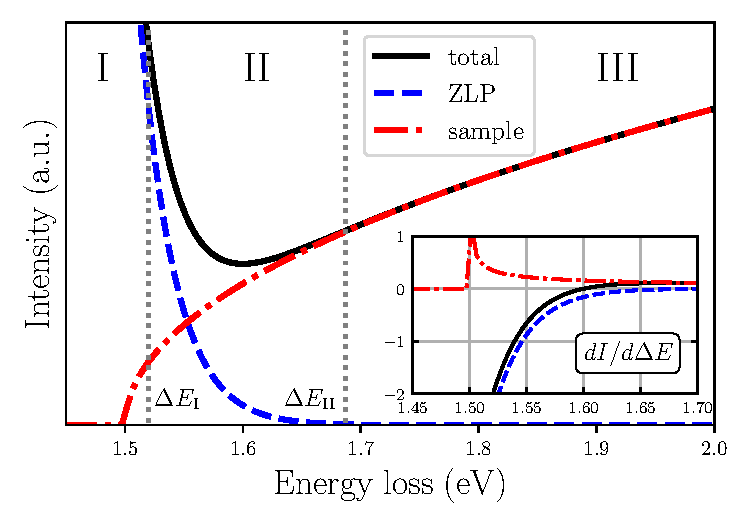
\includegraphics[width=0.89\textwidth]{plots/EELS_toy.pdf}
    \caption{A toy model for the EEL spectrum and its
      derivative (in the inset).
      %
      We display the separate contributions from $I_{\rm ZLP}$
      and $I_{\rm inel}$ as well as their sum.
      %
      We indicate the two regions used for the model training ($I$ and $III$),
      while as discussed in the text the trained model is then
      extrapolated to region $II$, defined for $\Delta E_I \le \Delta E \le \Delta E_{II}$.
    }
    \label{fig:EELS_toy}
\end{figure}
%%%%%%%%%%%%%%%%%%%%%%%%%%%%%%%%%%%%%%%%%%%%%%%%%

The toy model of Fig.~\ref{fig:EELS_toy} is general enough so that one can draw
a number of useful considerations concerning the relation between $I_{\rm ZLP}$ and $I_{\rm inel}$
in realistic spectra:

\begin{itemize}

\item The ZLP intensity, $I_{\rm ZLP}(\Delta E)$, is a monotonically decreasing function
  and thus its derivative is always negative.

\item  The first local minimum of the total spectrum, $dI_{\rm EELS}/d\Delta E|_{\Delta E_{\rm min}}=0$, corresponds
  to a value of $\Delta E$ for which the contribution from the inelastic emissions is already
  sizable.

\item The value of $\Delta E$ for which $I_{\rm inel}$ starts to contribute to the total spectrum
  corresponds to the position where the intensity derivatives in-sample and in-vacuum  start to differ.
  %
  We note that a direct comparison between the overal magnitude of the sample and vacuum ZLP
  spectra is in general not possible, as explained in Sect.~\ref{sec:eels}. 
\end{itemize}

These considerations suggest that when training the ML model on EEL spectra taken on samples,
the following categorisation should de adopted:

\begin{enumerate}

\item For energy losses such that $\Delta E \le \Delta E_I$ (region $I$),
  the model training  proceeds in the same way as for the vacuum case
  via the minimisation of Eq.~(\ref{eq:chi2})

\item  
  For $\Delta E \ge \Delta E_{II}$ (region $III$), we use instead Eq.~(\ref{eq:chi2modified})
  without the contribution from the input data, since for such values
  of $\Delta E$ one has that $I_{\rm inel}\gg I_{\rm ZLP}$.
  %
  In other words, the only information that the region $III$ provides
  on the model is the one arising from the implementation
  of the constraint that $I_{\rm ZLP}(\Delta E\to \infty)\to 0$.

\item The EELS data  in region $II$, defined by  $\Delta E_I \le \Delta E \le \Delta E_{II}$,
  is excluded from the training dataset, given that in this region the contribution to $I_{\rm EEL}$
  coming from $I_{\rm inel}$ is significant.
  %
  There the model predictions are obtained from an interpolation
  of the predictions obtained in regions $I$ and $III$.

\end{enumerate}

This classification introduces two new hyper-parameters of our model, $\Delta E_I$ and
$\Delta E_{II}$, that need to be specified before the training.
%
They should satisfy $\Delta E_I \le \Delta E_{\rm min}$ and $\Delta E_{II} \ge \Delta E_{\rm min}$,
with $\Delta E_{\rm min}$ being the position of the first local minimum of $I_{\rm EEL}$.
%
As indicated by the toy spectra of Fig.~\ref{fig:EELS_toy}, a suitable value for $\Delta E_{I}$
would be somewhat above the onset of the inelastic contributions, to maximise
the amount of training data while ensuring that $I_{\rm EEL}$ is dominated
by $I_{\rm ZLP}$.

We can use the derivatives of the spectra, $dI_{\rm EEL}/d\Delta E$, to select suitable minimum and
maximum values for $\Delta E_I$. In order to select the value for $\Delta E_{II}$, we use the intensity
profiles of the vacuum recorded spectra. 
%
Concerning $\Delta E_I $, its minimum possible value is selected as the value where the derivate taken on the sample
data start to different significantly as compared to those spectra taken on vacuum.
%
This value is obtained by looking at the ratio of the derivatives of the spectra compared to the vacuum derivatives,
$R_{dI/d \Delta E} =  \left( \frac{dI_{\rm ZLP}/d\Delta E}{dI_{\rm EEL}/d\Delta E}\right)$. 
%
For low energy losses this ratio equals 1, but at some energy loss $\Delta E_{I,min}$ the
sample stops monotonically decreasing and the ratio deviates from 1. 
%
We know that the hyper-parameter $\Delta E_I$ should satisfy $\Delta E_{I,min} \le \Delta E_I \le \Delta E_{\rm min}$,
which corresponds to the region where $R_{dI/d \Delta E} \ne  1$ and $R_{dI/d \Delta E} \ge 0$.
%
The neural network will be trained on an array of $\Delta E_I$ values within this interval and 
the optimal choice will be determined {\it a posteriori} from the results.
%
Another important difference as compared to the training of the vacuum spectra is that each of the sample
spectra will have different values of $\Delta E_{\rm min}$ and thus of $\Delta E_I$. 
%
For this reason we calculate $\Delta E_{\rm min}$  for each of the sample spectra and we use the highest of these
as the maximum value for the hyper-parameter $\Delta E_I$. 
%
As we determine the best choice of $\Delta E_I$ after training for each of the spectra separately, 
we are sure to capture all suitable results and select the best value for each individual spectrum. 
%
Concerning $\Delta E_{II}$, its minimum value should mark the region where $I_{\rm ZLP}(\Delta E\to \infty)\to 0$. 
%
In order to implement this constraint, similar to the previous section we look at the ratio 
$I_{ZLP,i}^{(exp)}/ \sigma_i^{(exp)}$ to determine the energy loss $\Delta E_{\rm pd}$ at 
which the contributions from the ZLP vanish. 
%
As a measure, we use the energy loss value where the ratio $I_{ZLP,io}^{(exp)}/\sigma_i^{(exp)}$ drops below 1. 
%
We set the value of $\Delta E_{II}$ equal to this energy loss and add pseudo-data points for $\Delta E \ge \Delta E_{II}$.
%
Note that in this region the intensity of the ZLP is several orders of magnitude smaller than the intensity 
of the elastic emissions and therefore the exact choice of $\Delta E_{II}$ doens't listen too closely.
